\documentclass[12pt, a4paper]{article}

%%% Поля
\usepackage[a4paper,top=1.5cm, bottom=1.5cm, left=2cm, right=2cm]{geometry}

%%% Кодировки и язык
\usepackage{cmap}                       % поиск в PDF
\usepackage{mathtext}                   % русские буквы в формулах
\usepackage[T2A]{fontenc}
\usepackage[utf8]{inputenc}
\usepackage[english,russian]{babel}

%%% Графика
\usepackage{graphicx}
\graphicspath{{images/}}
\DeclareGraphicsExtensions{.pdf,.png,.jpg}

%%% Цвета — ОБЯЗАТЕЛЬНО до hyperref!
\usepackage[rgb]{xcolor}

%%% Таблицы и обтекание
\usepackage{float}
\usepackage{wrapfig}
\usepackage{tabularx}
\usepackage{multirow}
\usepackage{array}
\usepackage{ragged2e}
\usepackage{enumitem}

%%% Подписи — ОБЯЗАТЕЛЬНО до hyperref
\usepackage{caption}
\usepackage{subcaption}

%%% Математика (один раз!)
\usepackage{amsmath,amsfonts,amssymb,amsthm,mathtools}
\usepackage{icomma}                     % умная запятая: $0,2$ — число
% \mathtoolsset{showonlyrefs=true}

%%% Шрифты и операторы
\usepackage{euscript}
\usepackage{mathrsfs}
% \usepackage[italicdiff]{physics}
\DeclareMathOperator{\sgn}{\mathop{sgn}}

%%% Переносы в формулах
\newcommand*{\hm}[1]{#1\nobreak\discretionary{}
{\hbox{$\mathsurround=0pt #1$}}{}}

%%% Красная абзацная строка
\usepackage{indentfirst}

%%% hyperref — ОДИН из последних!
\usepackage[unicode,
            colorlinks=true,
            urlcolor=blue,
            linkcolor=blue,
            citecolor=blue]{hyperref}

\usepackage{tikz}





\begin{document}



\include{titlepage}
\begin{titlepage}
\thispagestyle{empty}

\begin{center}
\small
Министерство науки и высшего образования Российской Федерации\\[2mm]
\textbf{ФЕДЕРАЛЬНОЕ ГОСУДАРСТВЕННОЕ АВТОНОМНОЕ
ОБРАЗОВАТЕЛЬНОЕ УЧРЕЖДЕНИЕ ВЫСШЕГО ОБРАЗОВАНИЯ}\\[1mm]
«МОСКОВСКИЙ ФИЗИКО-ТЕХНИЧЕСКИЙ ИНСТИТУТ\\
(НАЦИОНАЛЬНЫЙ ИССЛЕДОВАТЕЛЬСКИЙ УНИВЕРСИТЕТ)»\\
(МФТИ, Физтех)
\end{center}

\vspace{18mm}

\begin{center}
\large \textbf{КАФЕДРА ЭЛЕКТРОНИКИ}\\[10mm]
\Large \textbf{ОТЧЁТ}\\[2mm]
\large \textbf{ПО ЛАБОРАТОРНОЙ РАБОТЕ}\\[14mm]
\Large \textbf{АВТОЭЛЕКТРОННАЯ ЭМИССИЯ}
\end{center}

\vfill

% Блоки с подписями слева, линии и пояснения справа
\noindent
\begin{tabular}{@{}p{0.44\linewidth}p{0.52\linewidth}@{}}
\textit{Работу выполнили:} & Акимов Михаил,

Новиков Василий,

Рагозина Елизавета,

Струков Олег,

Топольский Михаил,

Группа Б04-404 \\[8mm]

\textit{Работу принял, оценка:} & \\[3mm]
 \\
\end{tabular}


\vspace{12mm}

\begin{center}
\small Долгопрудный, \the\year{}~г.
\end{center}

\end{titlepage}










\newpage


\section*{Теоретическая часть}

\subsection*{1. Физические основы автоэлектронной эмиссии}

Автоэлектронная эмиссия (автоэмиссия) -- явление испускания электронов в вакуум с поверхности твёрдого тела под действием сильного внешнего электрического поля напряжённостью $F \sim 10^{7}$--$10^{8}$~В/см. В отличие от термо-, фото- и вторичной эмиссии, при автоэмиссии не требуется подвод дополнительной энергии к электронам: выход электрона в вакуум обеспечивается за счёт туннелирования сквозь суженный поверхностный потенциальный барьер.

Основные преимущества автоэмиссионных катодов:
\begin{itemize}
    \item отсутствие накала;
    \item высокая плотность тока ($10^{3}$--$10^{6}$~А/см$^{2}$);
    \item малая инерционность отклика тока на изменение напряжения;
    \item устойчивость к колебаниям температуры и внешней радиации;
    \item высокая крутизна вольт-амперной характеристики (ВАХ) благодаря экспоненциальной зависимости тока от напряжения.
\end{itemize}

Для создания полей порядка $10^{7}$--$10^{8}$~В/см на макроскопических электродах потребовались бы напряжения в десятки мегавольт, поэтому на практике используют эмиттеры в виде острий с радиусом вершины $r \sim 10$--$1000$~нм. При микроскопических расстояниях катод--анод ($\sim$ единицы мкм) и малых радиусах кривизны ($r \sim 20$--$50$~\AA) автоэмиссию удаётся получить при напряжениях всего в сотни и даже десятки вольт.

\subsection*{2. Теория Фаулера--Нордгейма}

Впервые количественная теория автоэмиссии была построена Фаулером и Нордгеймом (1928~г.). Для плоского полубесконечного металла при $T = 0$~К, пренебрегая силами изображения, они получили выражение для плотности тока:
\begin{equation}
    j = A \frac{E^{2}}{\varphi}\exp\!\left(-B\frac{\varphi^{3/2}}{E}\right),
    \label{eq:FN}
\end{equation}
где $\varphi$ --- работа выхода, $E$ --- напряжённость электрического поля у поверхности, $A$ и $B$ --- универсальные константы.

С учётом сил электростатического изображения Нордгейм (1929~г.) модифицировал формулу:
\begin{equation}
    j = a\,\frac{E^{2}}{\varphi\,t^{2}(y)}\exp\!\left(-b\,\frac{\varphi^{3/2}}{E}\,v(y)\right),
    \label{eq:FN_nord}
\end{equation}
где $y = \sqrt{e^{3}E}/\varphi$, а $t(y)$ и $v(y)$ --- специальные функции Нордгейма, табулированные автором. При значениях аргумента, не близких к $0$ или $1$, функция $v(y)$ хорошо аппроксимируется аналитическим выражением, что позволяет привести (\ref{eq:FN_nord}) к виду
\begin{equation}
    j \approx a'\,\frac{E^{2}}{\varphi}\exp\!\left(-b'\,\frac{\varphi^{3/2}}{E}\right).
    \label{eq:FN_approx}
\end{equation}

Уравнение (\ref{eq:FN}) справедливо при $kT \ll \varphi$; при комнатной температуре $kT \approx 0{,}025$~эВ, а характерное значение $\varphi \approx 4$--$5$~эВ, поэтому условие выполняется с запасом. Более общая теория, объединяющая термо- и автоэлектронную эмиссию, была построена Мерфи и Гудом (1956~г.). В пределе низких температур их формула переходит в уравнение Фаулера--Нордгейма.

Подставляя численные значения констант, получаем практическую формулу (при $E$ в~В/см, $\varphi$ в~эВ, $j$ в~А/см$^{2}$):
\begin{equation}
    j = 1{,}54\cdot10^{-6}\,\frac{E^{2}}{\varphi\,t^{2}(y)}\,
    \exp\!\left(-6{,}83\cdot10^{7}\,\frac{\varphi^{3/2}}{E}\,v(y)\right).
    \label{eq:FN_num}
\end{equation}

\subsection*{3. Координаты Фаулера--Нордгейма}

Если построить зависимость $\ln(j/E^{2})$ от $1/E$, то в узком диапазоне полей получается практически прямая линия --- \textit{график Фаулера--Нордгейма}. Наклон этой прямой определяется выражением
\begin{equation}
    \tg\alpha = -\,b\,\varphi^{3/2}\,s(y),
    \label{eq:slope}
\end{equation}
где $s(y)$ --- ещё одна спецфункция Нордгейма. В рабочем диапазоне её можно считать приблизительно постоянной ($s \approx 1$), что позволяет по наклону прямой находить работу выхода $\varphi$ (или, наоборот, напряжённость поля $E$).

\subsection*{4. Одно- и многоэмиттерные системы}

На практике измеряют не плотность тока $j$, а полный ток $I$ при приложенном напряжении $U$. Связь между ними устанавливается через площадь эмиттера $S_{\text{э}}$ и \textit{форм-фактор} острия $\beta$:
\begin{equation}
    I = S_{\text{э}}\,j, \qquad E = \beta\,U.
\end{equation}
Тогда уравнение Фаулера--Нордгейма для полного тока принимает вид
\begin{equation}
    I = A_{FN}\,\frac{(\beta U)^{2}}{\varphi}\exp\!\left(-B_{FN}\,\frac{\varphi^{3/2}}{\beta U}\right),
    \label{eq:FN_IU}
\end{equation}
где $A_{FN}$ и $B_{FN}$ --- константы, зависящие от площади эмиттера.

Для \textit{многоэмиттерных} систем (например, пучков углеродных волокон), содержащих $N$ эмиссионных центров, суммарный ток в первом приближении (без учёта экранировки) равен
\begin{equation}
    I = \sum_{i=1}^{N} I_{i}.
\end{equation}
При малом разбросе форм-факторов центров после тренировки катода можно ввести средний форм-фактор $\bar\beta$, и тогда
\begin{equation}
    I = N\,A_{FN}\,\frac{(\bar\beta U)^{2}}{\varphi}\exp\!\left(-B_{FN}\,\frac{\varphi^{3/2}}{\bar\beta U}\right).
    \label{eq:FN_multi}
\end{equation}
Суммарная площадь рабочей поверхности $S = N\,k\,\pi r^{2}$, где $r$ --- характерный размер центра, $k$ --- коэффициент, зависящий от формы центра.

\subsection*{5. Нестабильность автоэмиссионного тока}

Основные причины нестабильности тока автоэмиссионных катодов:
\begin{enumerate}
    \item ионная бомбардировка поверхности ионами остаточных газов, изменяющая микрогеометрию центров;
    \item адсорбция и десорбция атомов остаточных газов, меняющая локальную работу выхода;
    \item разрушение центров под действием пондеромоторных сил;
    \item перегрев центров при больших плотностях тока;
    \item механическая непрочность катода и электростатическое отталкивание элементов.
\end{enumerate}

В рамках модели (\ref{eq:FN_multi}) ток может меняться при изменении радиуса центров $r$, работы выхода $\varphi$ и числа центров $N$. Сравнивая выражения для тока в разные моменты времени, можно качественно определить доминирующий механизм нестабильности, снимая ВАХ через малые промежутки времени и строя зависимость $\ln(I_{2}/I_{1})$ от $\ln(U_{2}/U_{1})$ (или аналогичные координаты):
\begin{itemize}
    \item если флуктуации обусловлены изменением числа центров $N$, то наклон прямой меняется, а свободный член остаётся постоянным;
    \item если причина --- изменение работы выхода $\varphi$, то зависимость линейна с коэффициентом пропорциональности $1{,}5$;
    \item если причина --- изменение размеров центров $r$, то линейный характер наблюдается в координатах от $1/U$.
\end{itemize}
При одновременном действии нескольких механизмов однозначная интерпретация затруднена, но можно качественно оценить вклад каждого.

\subsection*{6. Автоэлектронная микроскопия}

Автоэлектронный микроскоп (проектор Мюллера, 1937~г.) позволяет визуализировать распределение работы выхода и локальной напряжённости поля по поверхности острия. Электроны, эмитированные практически перпендикулярно поверхности, ускоряются полем и попадают на люминесцентный экран, формируя увеличенное изображение эмиттера.

Увеличение микроскопа определяется геометрией:
\begin{equation}
    M = \frac{R}{\gamma\,r},
    \label{eq:magnification}
\end{equation}
где $R$ --- расстояние эмиттер--экран, $\gamma \approx 1{,}5$--$1{,}9$ --- фактор сжатия, $r$ --- радиус острия. Для острия с $r < 0{,}5$~мкм и $R \approx 100$~мм увеличение достигает $10^{5}$.

Разрешение микроскопа ограничено длиной волны де Бройля эмитированных электронов и тангенциальными компонентами их скоростей (уровень Ферми соответствует эффективным температурам в тысячи кельвинов). Предельное разрешение составляет около $20$~\AA, и охлаждение образца этот предел не улучшает.

На автоэмиссионном изображении монокристаллического острия тёмные участки соответствуют плотноупакованным граням с большой работой выхода (например, (110), (100)), а светлые --- граням с меньшей работой выхода. Это позволяет определять кристаллографические индексы граней и изучать процессы адсорбции, фазовых превращений и роста плёнок на поверхности.

\subsection*{7. Автоэмиссионные свойства углеродных материалов}

Наиболее подходящими для создания стабильных автокатодов в условиях высокого технического вакуума оказались графит и полиакрилонитрильные углеродные волокна. Их структура состоит из фибрилл (размер по большой оси $L_{a} \sim 1000$~нм, диаметр $L_{c} \sim 50$~нм), связанных аморфными областями, что обеспечивает эластичность волокон. Эмиссионными центрами служат многочисленные ($\sim 10^{5}$) микровыступы на торцевой поверхности волокна. Разрушение отдельных микровыступов не приводит к существенному падению тока, так как среднее число активных центров остаётся постоянным -- это обеспечивает высокую стабильность и большой срок службы катода.

Для выравнивания электрического поля по пучку волокон и устранения выступающих волокон применяется травление коронным разрядом на воздухе. Отрицательная корона на катоде вызывает бомбардировку поверхности ионами кислорода и окисление углерода. В результате «выступающие» волокна стравливаются быстрее, периферийные --- укорачиваются, и пучок приобретает закруглённую геометрическую форму, что приводит к более равномерной эмиссии в вакууме.










\section*{Ход работы}

\subsection*{Схема установки}

Экспериментальная установка для исследования автоэмиссионных свойств катода собрана по схеме, изображённой на рис.~\ref{fig:setup}.

\begin{figure}[H]
\centering
% Раскомментируй строку ниже, когда добавишь схему
% \includegraphics[width=0.85\textwidth]{images/setup_scheme.pdf}
\rule{0.85\textwidth}{0.4\textwidth} % Временная заглушка
\caption{Электрическая схема экспериментальной установки}
\label{fig:setup}
\end{figure}

Установка содержит три параллельные ветви:
\begin{enumerate}
    \item \textbf{Ветвь источника высокого напряжения.} Низкое напряжение от лабораторного источника питания подаётся на умножитель напряжения, увеличивающий его в 1000 раз. Таким образом, при напряжениях источника порядка единиц вольт на выходе умножителя формируются потенциалы в единицы киловольт, необходимые для возбуждения автоэлектронной эмиссии.
    \item \textbf{Измерительная ветвь напряжения.} Высокое напряжение с выхода умножителя подаётся на делитель напряжения с коэффициентом деления $1/1000$. Напряжение после делителя измеряется вольтметром (осциллографом).% Зная показания вольтметра $U_{\text{в}}$, истинное напряжение на лампе вычисляется как $U = 1000 \cdot U_{\text{в}}$.
    \item \textbf{Измерительная ветвь тока.} Ток, эмитированный с катода лампы, протекает через амперметр, включённый последовательно в цепь катода, и возвращается на отрицательный полюс умножителя (землю).
\end{enumerate}

% Все три ветви подключены параллельно к общим шинам: положительная шина -- к аноду лампы и входу делителя, отрицательная -- к катоду (через амперметр) и выходу делителя.

\subsection*{Устройство автоэмиссионной лампы}

Исследуемый образец представляет собой отпаянную стеклянную лампу с автоэмиссионным катодом на основе пучка углеродных волокон. Конструкция лампы показана на рис.~\ref{fig:lamp}.

\begin{figure}[H]
\centering
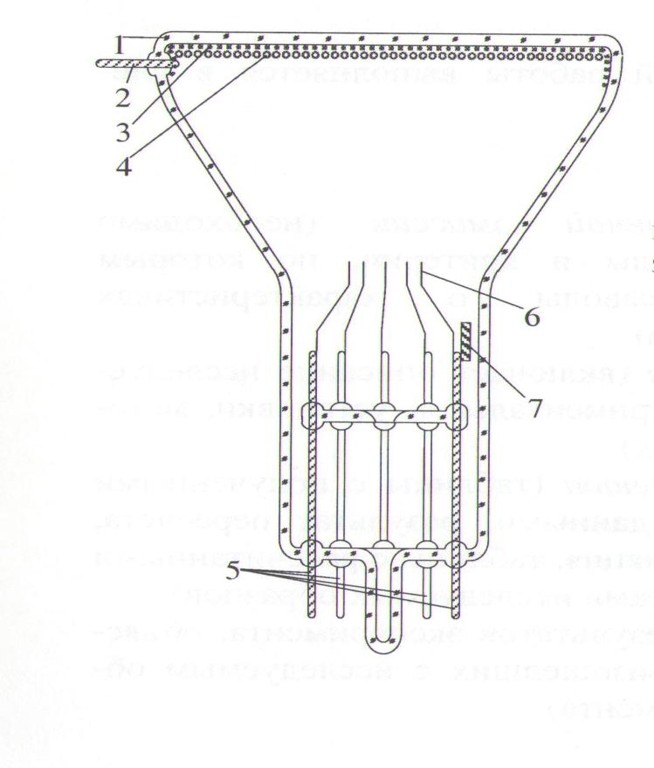
\includegraphics[width=0.45\textwidth]{1.jpg}
\caption{Конструкция автоэмиссионной лампы на основе углеродных волокон: 
1~--- стеклянная колба, 2~--- высоковольтный вывод, 3~--- проводящее покрытие (анод), 
4~--- люминофор, 5~--- катодные выводы, 6~--- автоэмиссионный катод (пучок углеродных волокон), 
7~--- геттер}
\label{fig:lamp}
\end{figure}

% Лампа состоит из следующих элементов:
% \begin{itemize}
%     \item \textbf{Стеклянная колба (1)} --- герметичный корпус, внутри которого поддерживается высокий вакуум.
%     \item \textbf{Высоковольтный вывод (2)} --- обеспечивает подвод высокого напряжения от умножителя к аноду лампы.
%     \item \textbf{Проводящее покрытие (3)} --- нанесено на внутреннюю поверхность колбы (обычно $\text{SnO}_2$ или $\text{In}_2\text{O}_3$) и служит анодом.
%     \item \textbf{Люминофор (4)} --- слой люминесцентного материала поверх проводящего покрытия; светится при попадании на него ускоренных электронов, формируя автоэмиссионное изображение.
%     \item \textbf{Катодные выводы (5)} --- держатели, на которых закреплён автоэмиссионный катод.
%     \item \textbf{Автоэмиссионный катод (6)} --- пучок полиакрилонитрильных углеродных волокон, предварительно подвергнутый травлению коронным разрядом на воздухе для выравнивания электрического поля и устранения выступающих волокон.
%     \item \textbf{Геттер (7)} --- поглотитель остаточных газов, поддерживающий высокий вакуум в колбе в течение всего срока службы лампы.
% \end{itemize}

Испытания лампы проводятся в \textbf{диодном режиме}: на анод (проводящее покрытие) подаётся положительное высокое напряжение, катод заземлён через амперметр. Электроны, эмитированные с острий углеродных волокон под действием сильного электрического поля, ускоряются в зазоре катод--анод и попадают на люминофор, вызывая его свечение. Расстояние катод--анод (радиус колбы) составляет порядка нескольких сантиметров, что в сочетании с микроскопическими радиусами вершин волокон ($r \sim 10$--$100$~нм) обеспечивает напряжённость поля у поверхности эмиттера $E \sim 10^{7}$--$10^{8}$~В/см при приложенных напряжениях в единицы киловольт.


\section*{Результаты измерений}

\subsection*{1. Измерение ВАХ}

В ходе эксперимента была снята вольт-амперная характеристика (ВАХ) автоэмиссионного катода на основе пучка углеродных волокон. Погрешности прямых измерений составляют:
\begin{itemize}
    \item абсолютная погрешность напряжения на лампе: $\Delta U = 0{,}01$~кВ;
    \item относительная погрешность измерения тока: $\delta I = 2{,}5\,\%$.
\end{itemize}

Результаты ручных измерений представлены в таблице~\ref{tab:raw_data}.

\begin{table}[H]
\centering
\caption{Вольт-амперная характеристика автоэмиссионного катода (ручные измерения)}
\label{tab:raw_data}
\begin{tabular}{|c|c|c|}
\hline
$U_{\text{вх}}$, В & $U$, кВ & $I$, мкА \\
\hline
6,6  & 1,52 & 4,25  \\
6,7  & 1,54 & 5,25  \\
7,0  & 1,60 & 9,75  \\
7,2  & 1,63 & 16,25 \\
7,3  & 1,65 & 19,38 \\
7,4  & 1,67 & 22,50 \\
7,5  & 1,68 & 26,25 \\
7,7  & 1,71 & 33,75 \\
7,9  & 1,74 & 42,50 \\
8,1  & 1,76 & 52,50 \\
8,3  & 1,79 & 62,50 \\
8,5  & 1,82 & 72,50 \\
8,7  & 1,84 & 85,00 \\
\hline
\end{tabular}
\end{table}

На рисунке~\ref{fig:manual_IV} представлена вольт-амперная характеристика в исходных координатах.

\begin{figure}[H]
\centering
% Убедись, что имя файла совпадает с тем, что сгенерировал Python (например, manual_IV.pdf или 5.pdf)
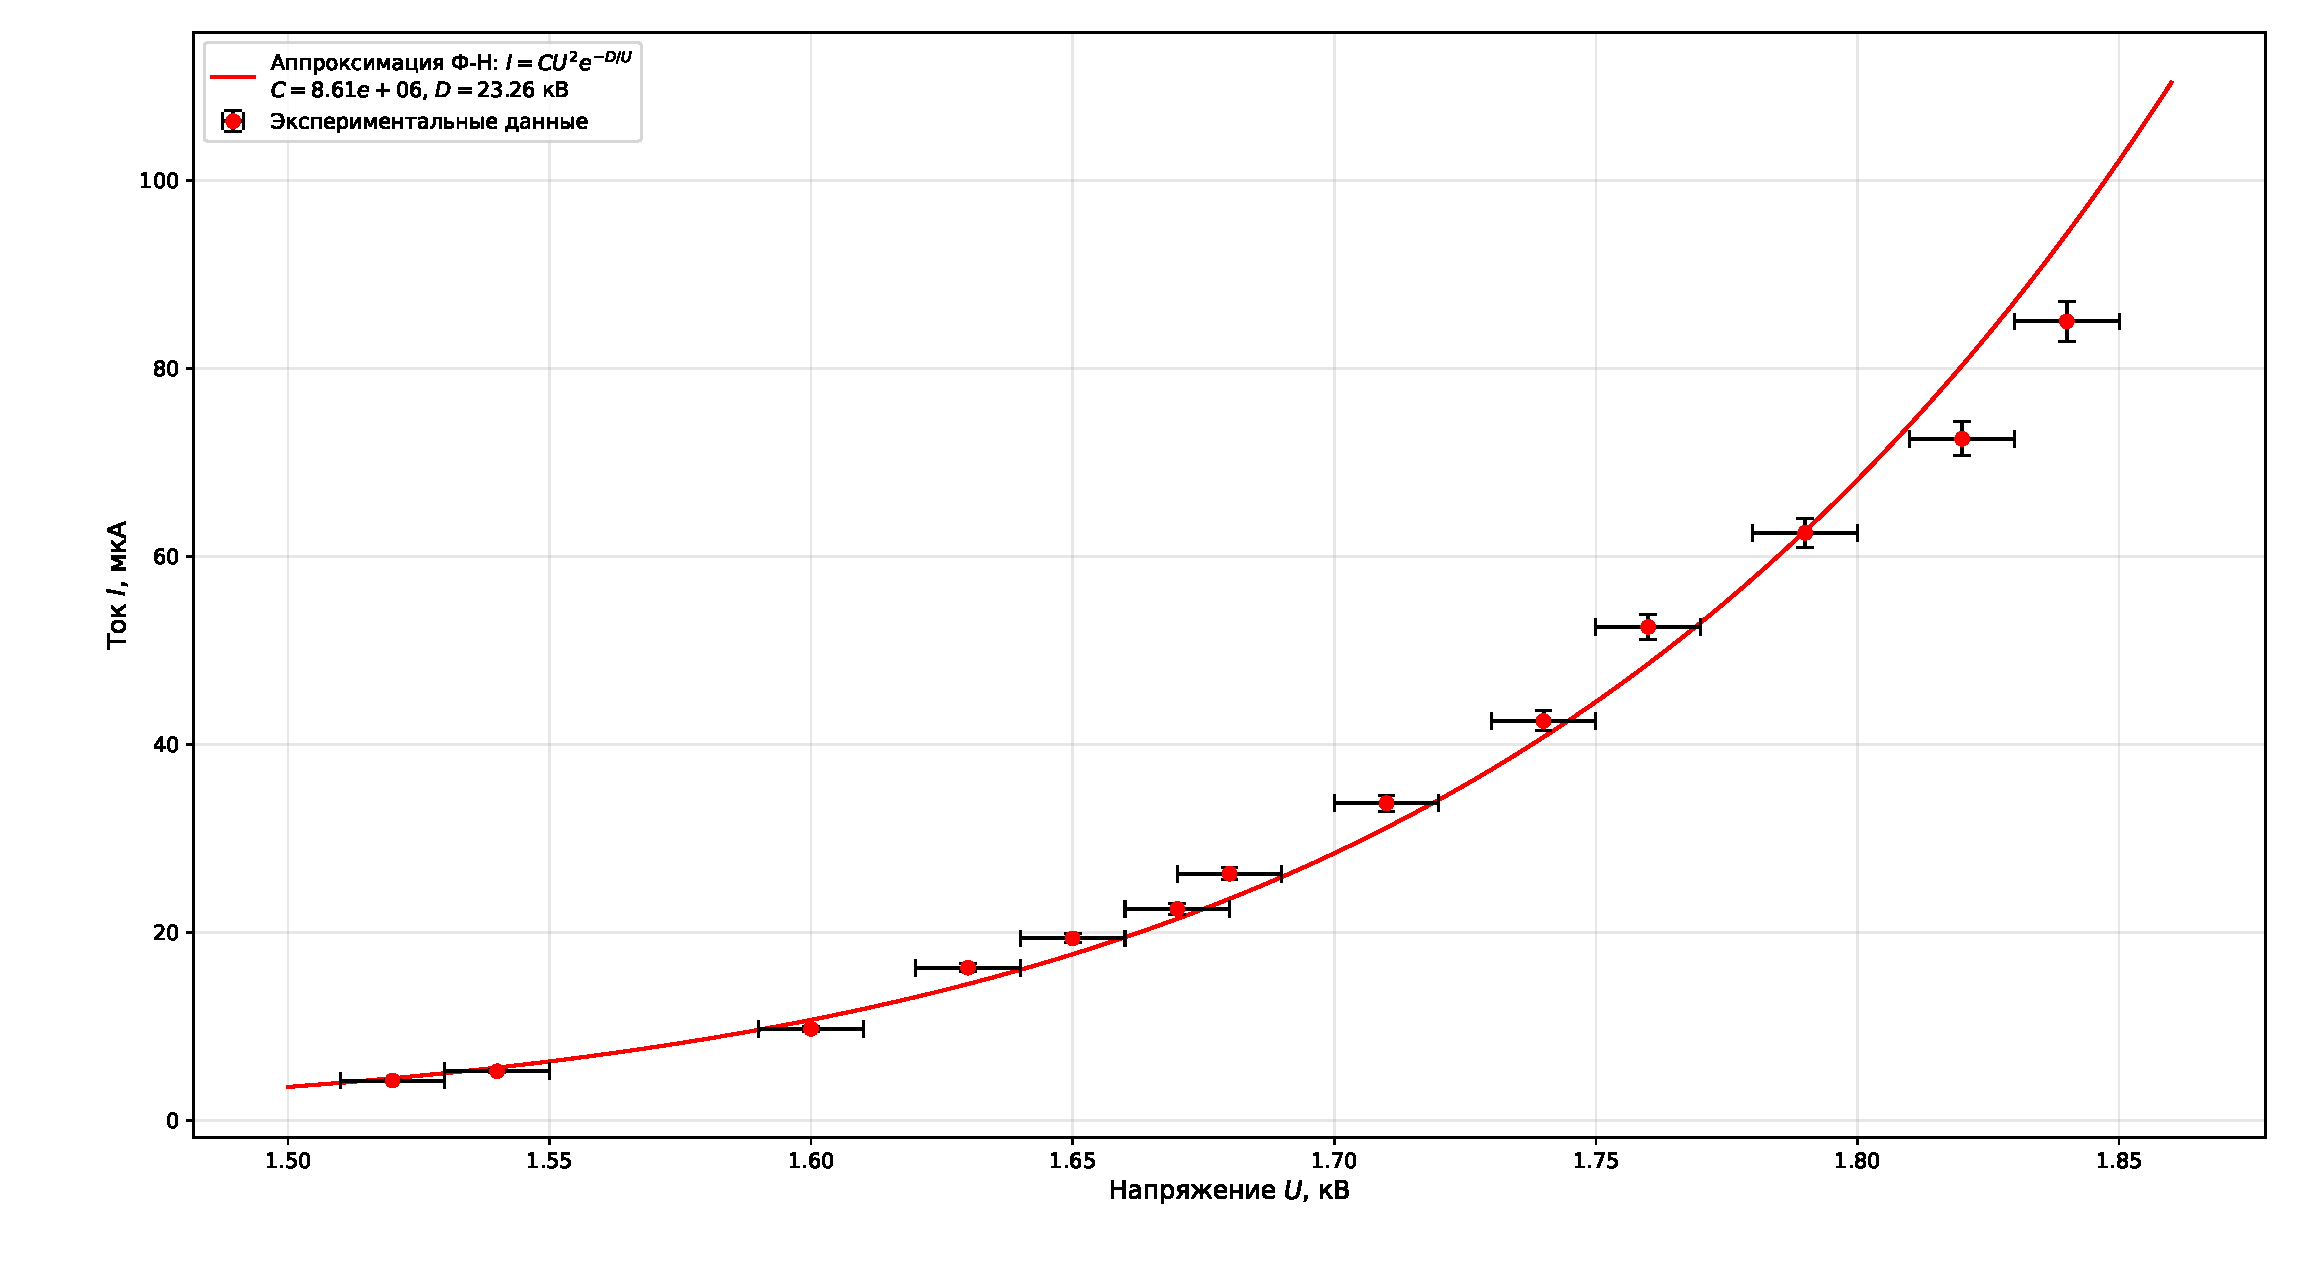
\includegraphics[width=0.8\textwidth]{5.pdf} 
\caption{Вольт-амперная характеристика автоэмиссионного катода (ручные измерения)}
\label{fig:manual_IV}
\end{figure}

\subsection*{2. Обработка данных в координатах Фаулера--Нордгейма}

Для определения параметров эмиттера экспериментальные данные были пересчитаны в координаты Фаулера--Нордгейма. Уравнение Фаулера--Нордгейма для полного тока имеет вид:
\begin{equation}
    I = A\,\frac{(\beta U)^{2}}{\varphi}\,
    \exp\!\left(-B\,\frac{\varphi^{3/2}}{\beta\,U}\right),
    \label{eq:FN_IU}
\end{equation}
где $U$ --- приложенное напряжение (В), $\varphi$ --- работа выхода (эВ), $\beta$ --- форм-фактор острия (см$^{-1}$), $B = 6{,}83\cdot10^{7}$~В$\cdot$см$^{-1}\cdot$эВ$^{-3/2}$.

Прологарифмировав (\ref{eq:FN_IU}) и разделив на $U^{2}$, получаем линейную зависимость:
\begin{equation}
    \ln\!\left(\frac{I}{U^{2}}\right) = \ln\!\left(\frac{A\,\beta^{2}}{\varphi}\right) 
    - \frac{B\,\varphi^{3/2}}{\beta}\cdot\frac{1}{U}.
    \label{eq:FN_linear}
\end{equation}

Таким образом, в координатах $\bigl(1/U,\;\ln(I/U^{2})\bigr)$ экспериментальные точки должны выстраиваться в прямую линию с наклоном
\begin{equation}
    k = -\frac{B\,\varphi^{3/2}}{\beta}.
    \label{eq:slope}
\end{equation}

На рисунке~\ref{fig:fn_plot} представлена вольт-амперная характеристика в координатах Фаулера--Нордгейма.
%  Погрешности по оси ординат рассчитаны по формуле передачи ошибок:
% \begin{equation}
%     \Delta\!\left[\ln\!\left(\frac{I}{U^{2}}\right)\right] 
%     = \sqrt{\delta I^{2} + \left(\frac{2\,\Delta U}{U}\right)^{2}}.
% \end{equation}

Линейная аппроксимация экспериментальных точек методом наименьших квадратов дала значение наклона прямой $k$, по которому далее определялся форм-фактор $\beta$.

\begin{figure}[H]
\centering
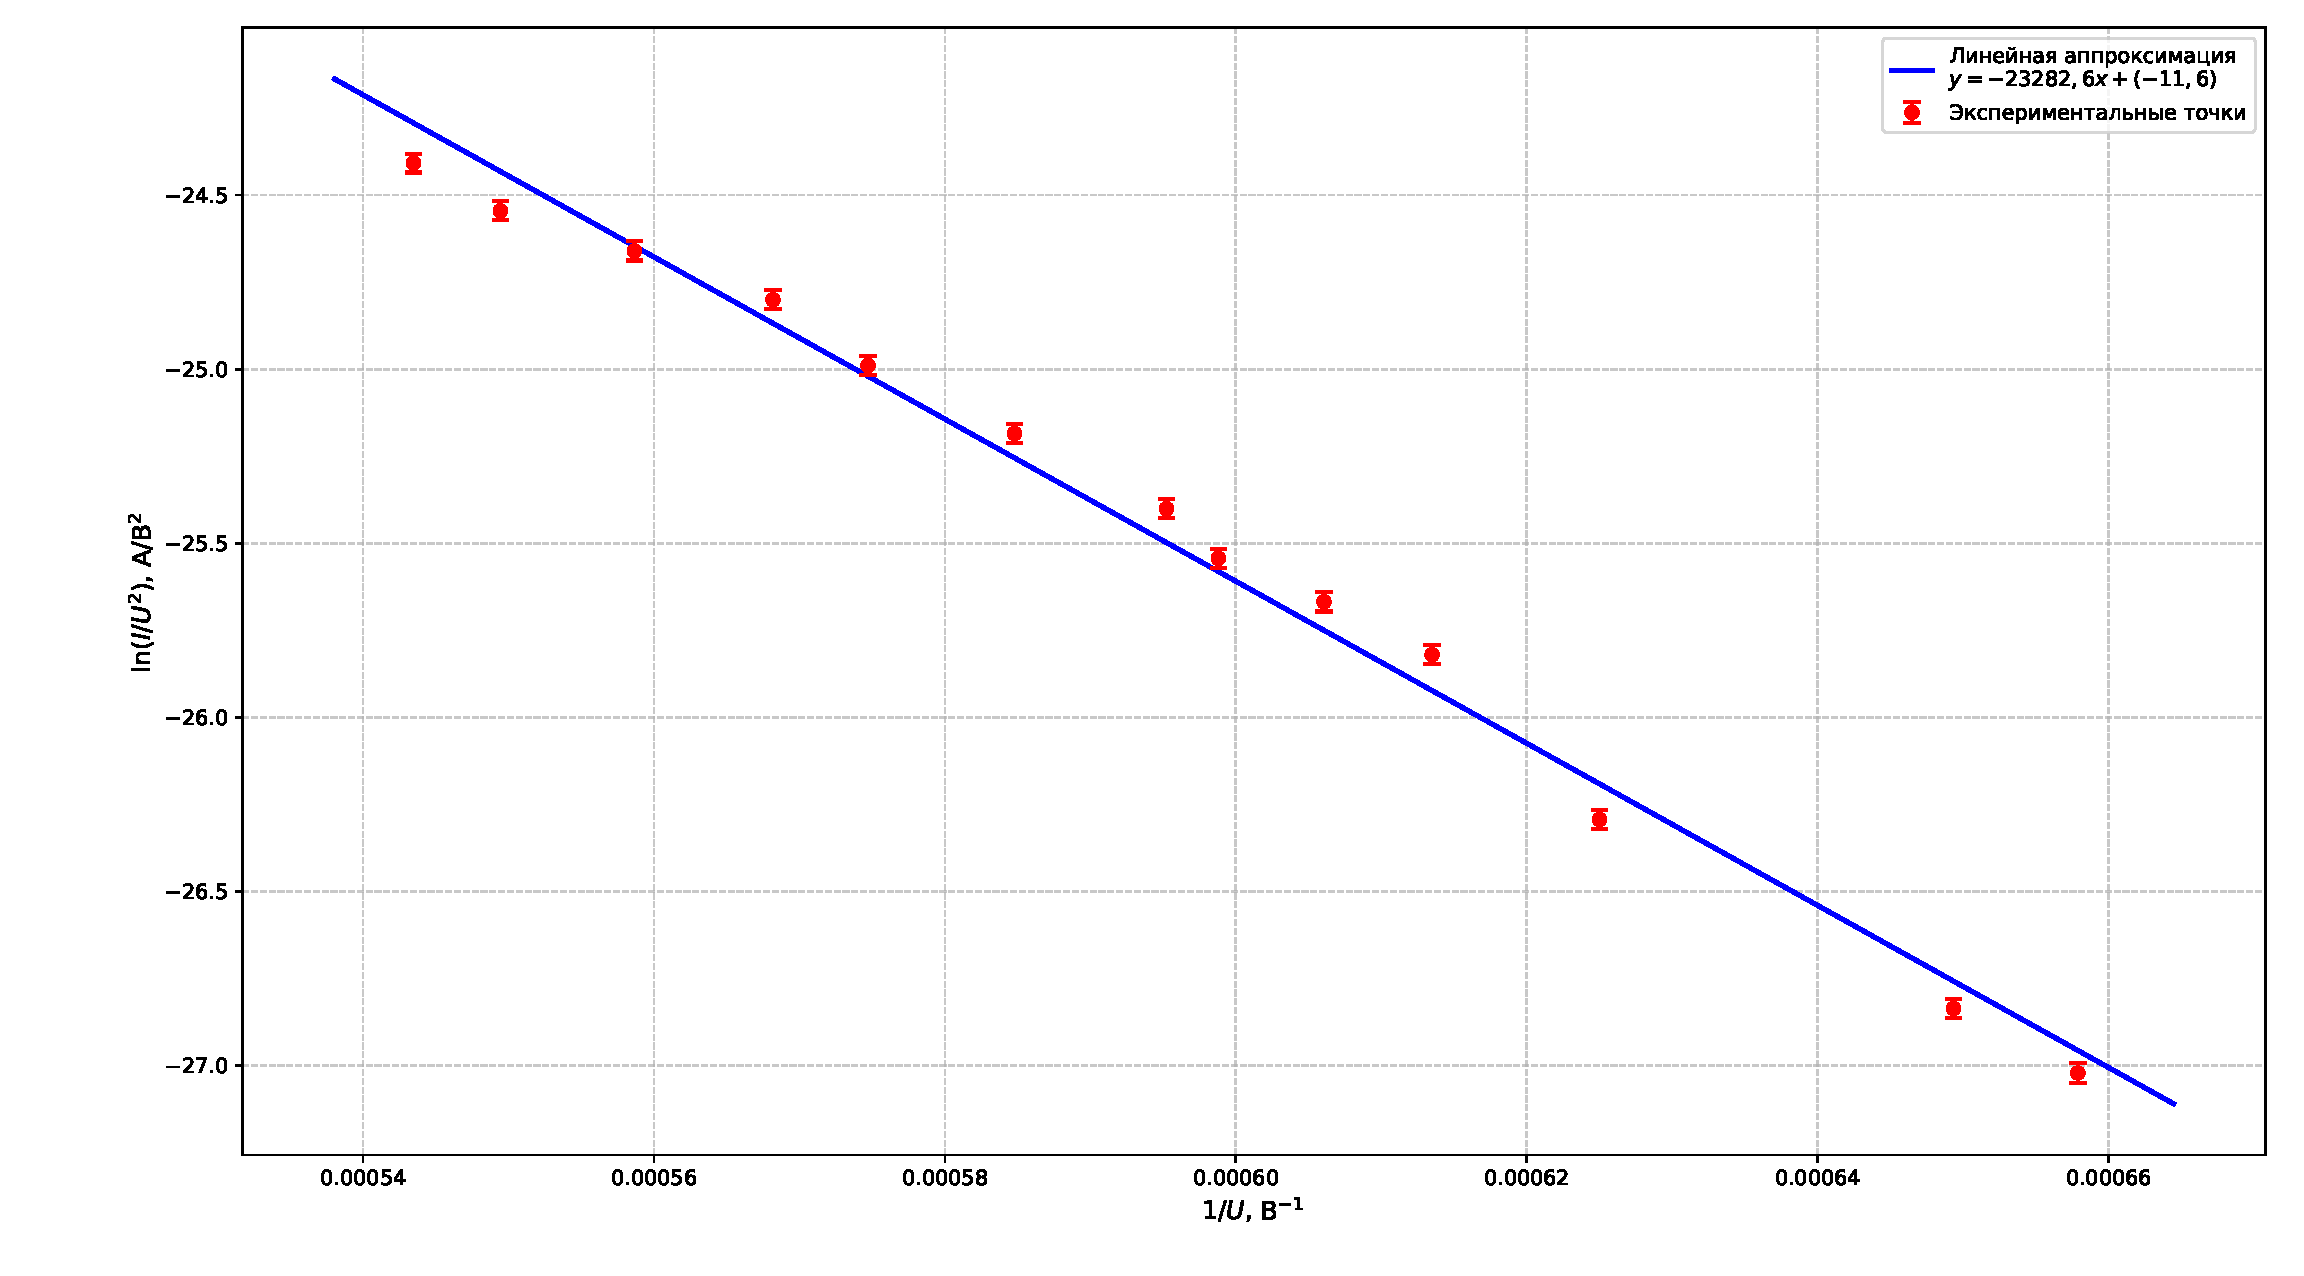
\includegraphics[width=0.85\textwidth]{2.pdf}
\caption{Вольт-амперная характеристика в координатах Фаулера--Нордгейма (ручные измерения). 
Красные точки --- экспериментальные данные с погрешностями, 
синяя линия --- линейная аппроксимация}
\label{fig:fn_plot}
\end{figure}

\subsection*{3. Расчёт параметров эмиттера}

Для расчёта геометрических параметров катода использовались следующие значения:
\begin{itemize}
    \item работа выхода углеродного материала: $\varphi = 4{,}7$~эВ;
    \item расстояние катод--анод: $R = 1$~мм $= 0{,}1$~см;
    \item геометрический коэффициент для параболического центра: $k_{\text{г}} = 1/2$;
    \item фактор сжатия автоэлектронного микроскопа: $\gamma = 1{,}7$.
\end{itemize}

\textbf{Форм-фактор острия $\beta$.} Из выражения (\ref{eq:slope}) находим:
\begin{equation}
    \beta = -\frac{B\,\varphi^{3/2}}{k}.
    \label{eq:beta}
\end{equation}

\textbf{Характерный радиус эмиттирующего центра $r$.} 
Величина $r$ находилась численным решением трансцендентного уравнения:
\begin{equation}
    \beta = \frac{1}{k \cdot r \cdot \ln(R/r)},
    \label{eq:r_transcendental}
\end{equation}
при известных значениях $\beta$, $R = 1$~мм и $k = 1/2$.

\textbf{Коэффициент увеличения автоэлектронного микроскопа $M$.} Определяется геометрией установки:
\begin{equation}
    M = \frac{R}{\gamma\,r}.
    \label{eq:M}
\end{equation}

% \textbf{Погрешности.} Погрешность форм-фактора определялась как
% \begin{equation}
%     \frac{\Delta\beta}{\beta} = \sqrt{\left(\frac{\Delta k}{k}\right)^{2} 
%     + \left(\frac{1{,}5\,\Delta\varphi}{\varphi}\right)^{2}},
% \end{equation}
% где $\Delta k$ --- стандартная ошибка наклона из линейной регрессии, $\Delta\varphi = 0{,}1$~эВ. Погрешности радиуса и коэффициента увеличения находились по стандартным формулам передачи ошибок:
% \begin{equation}
%     \frac{\Delta r}{r} = \sqrt{\left(\frac{\Delta R}{R}\right)^{2} 
%     + \left(\frac{\Delta\beta}{\beta}\right)^{2}}, \qquad
%     \frac{\Delta M}{M} = \sqrt{\left(\frac{\Delta R}{R}\right)^{2} 
%     + \left(\frac{\Delta r}{r}\right)^{2} 
%     + \left(\frac{\Delta\gamma}{\gamma}\right)^{2}},
% \end{equation}
% где $\Delta R = 0{,}01$~см, $\Delta\gamma = 0{,}2$.

\subsection*{4. Результаты вычислений}

По результатам обработки вольт-амперной характеристики получены следующие параметры автоэмиссионного катода на основе углеродных волокон:

\begin{table}[H]
\centering
\caption{Параметры автоэмиссионного катода}
\label{tab:results}
\begin{tabular}{|l|c|}
\hline
Параметр & Значение \\
\hline
Форм-фактор острия $\beta$ & $(2{,}99 \pm 0{,}13)\cdot10^{4}$~см$^{-1}$ \\
Радиус закругления эмиттирующего центра $r$ & $67 \pm 7$~нм \\
Коэффициент увеличения микроскопа $M$ & $(8{,}8 \pm 1{,}7)\cdot10^{3}$ \\
\hline
\end{tabular}
\end{table}

Полученные значения форм-фактора и радиуса закругления соответствуют типичным параметрам эмиссионных центров на торцевой поверхности пучка полиакрилонитрильных углеродных волокон: микровыступы размером порядка десятков нанометров обеспечивают усиление электрического поля в $\sim 3\cdot10^{4}$ раз, что позволяет возбуждать автоэмиссию при напряжениях порядка единиц киловольт на межэлектродном расстоянии $1$~мм. %Коэффициент увеличения автоэлектронного микроскопа составляет порядка $10^{4}$, что согласуется с оценками для острий с радиусом кривизны $\sim 10^{-5}$~см и расстоянием катод--экран $\sim 1$~мм.


\subsection*{5. Исследование переходных процессов и автоматические измерения}

Для исследования динамики автоэмиссионного тока при включении высокого напряжения схема установки была изменена. Амперметр был заменён на два последовательно соединённых резистора: нагрузочный с сопротивлением $R_{\text{н}} = 1{,}08$~кОм и измерительный с сопротивлением $R_{\text{изм}} = 21{,}7$~кОм. Напряжение на измерительном резисторе регистрировалось цифровым осциллографом.

\begin{figure}[H]
\centering
% \includegraphics[width=0.85\textwidth]{images/setup_stage2.pdf}
\rule{0.85\textwidth}{0.4\textwidth}
\caption{Электрическая схема установки для второго этапа эксперимента}
\label{fig:setup_stage2}
\end{figure}


Ток через катод лампы в каждый момент времени рассчитывался по закону Ома:
\begin{equation}
    I(t) = \frac{U(t)}{R_{\text{изм}}},
    \label{eq:current_calc}
\end{equation}

Эксперимент заключался в подаче фиксированного напряжения на четыре различных катода на основе углеродных волокон и регистрации осциллограмм нарастания тока и напряжения в течение $1$~с с частотой дискретизации $2{,}5$~кГц. Параметры регистрации осциллографа:
\begin{itemize}
    \item частота дискретизации: $2{,}5$~кГц (интервал между точками $0{,}4$~мс);
    \item вертикальная развёртка: $0{,}5$~В/дел (канал 3);
    \item горизонтальная развёртка: $0{,}1$~с/дел;
    \item длина записи: $2500$ точек.
\end{itemize}

На рисунке~\ref{fig:transient} представлены полученные зависимости тока и напряжения для четырёх исследованных катодов.

\begin{figure}[H]
\centering
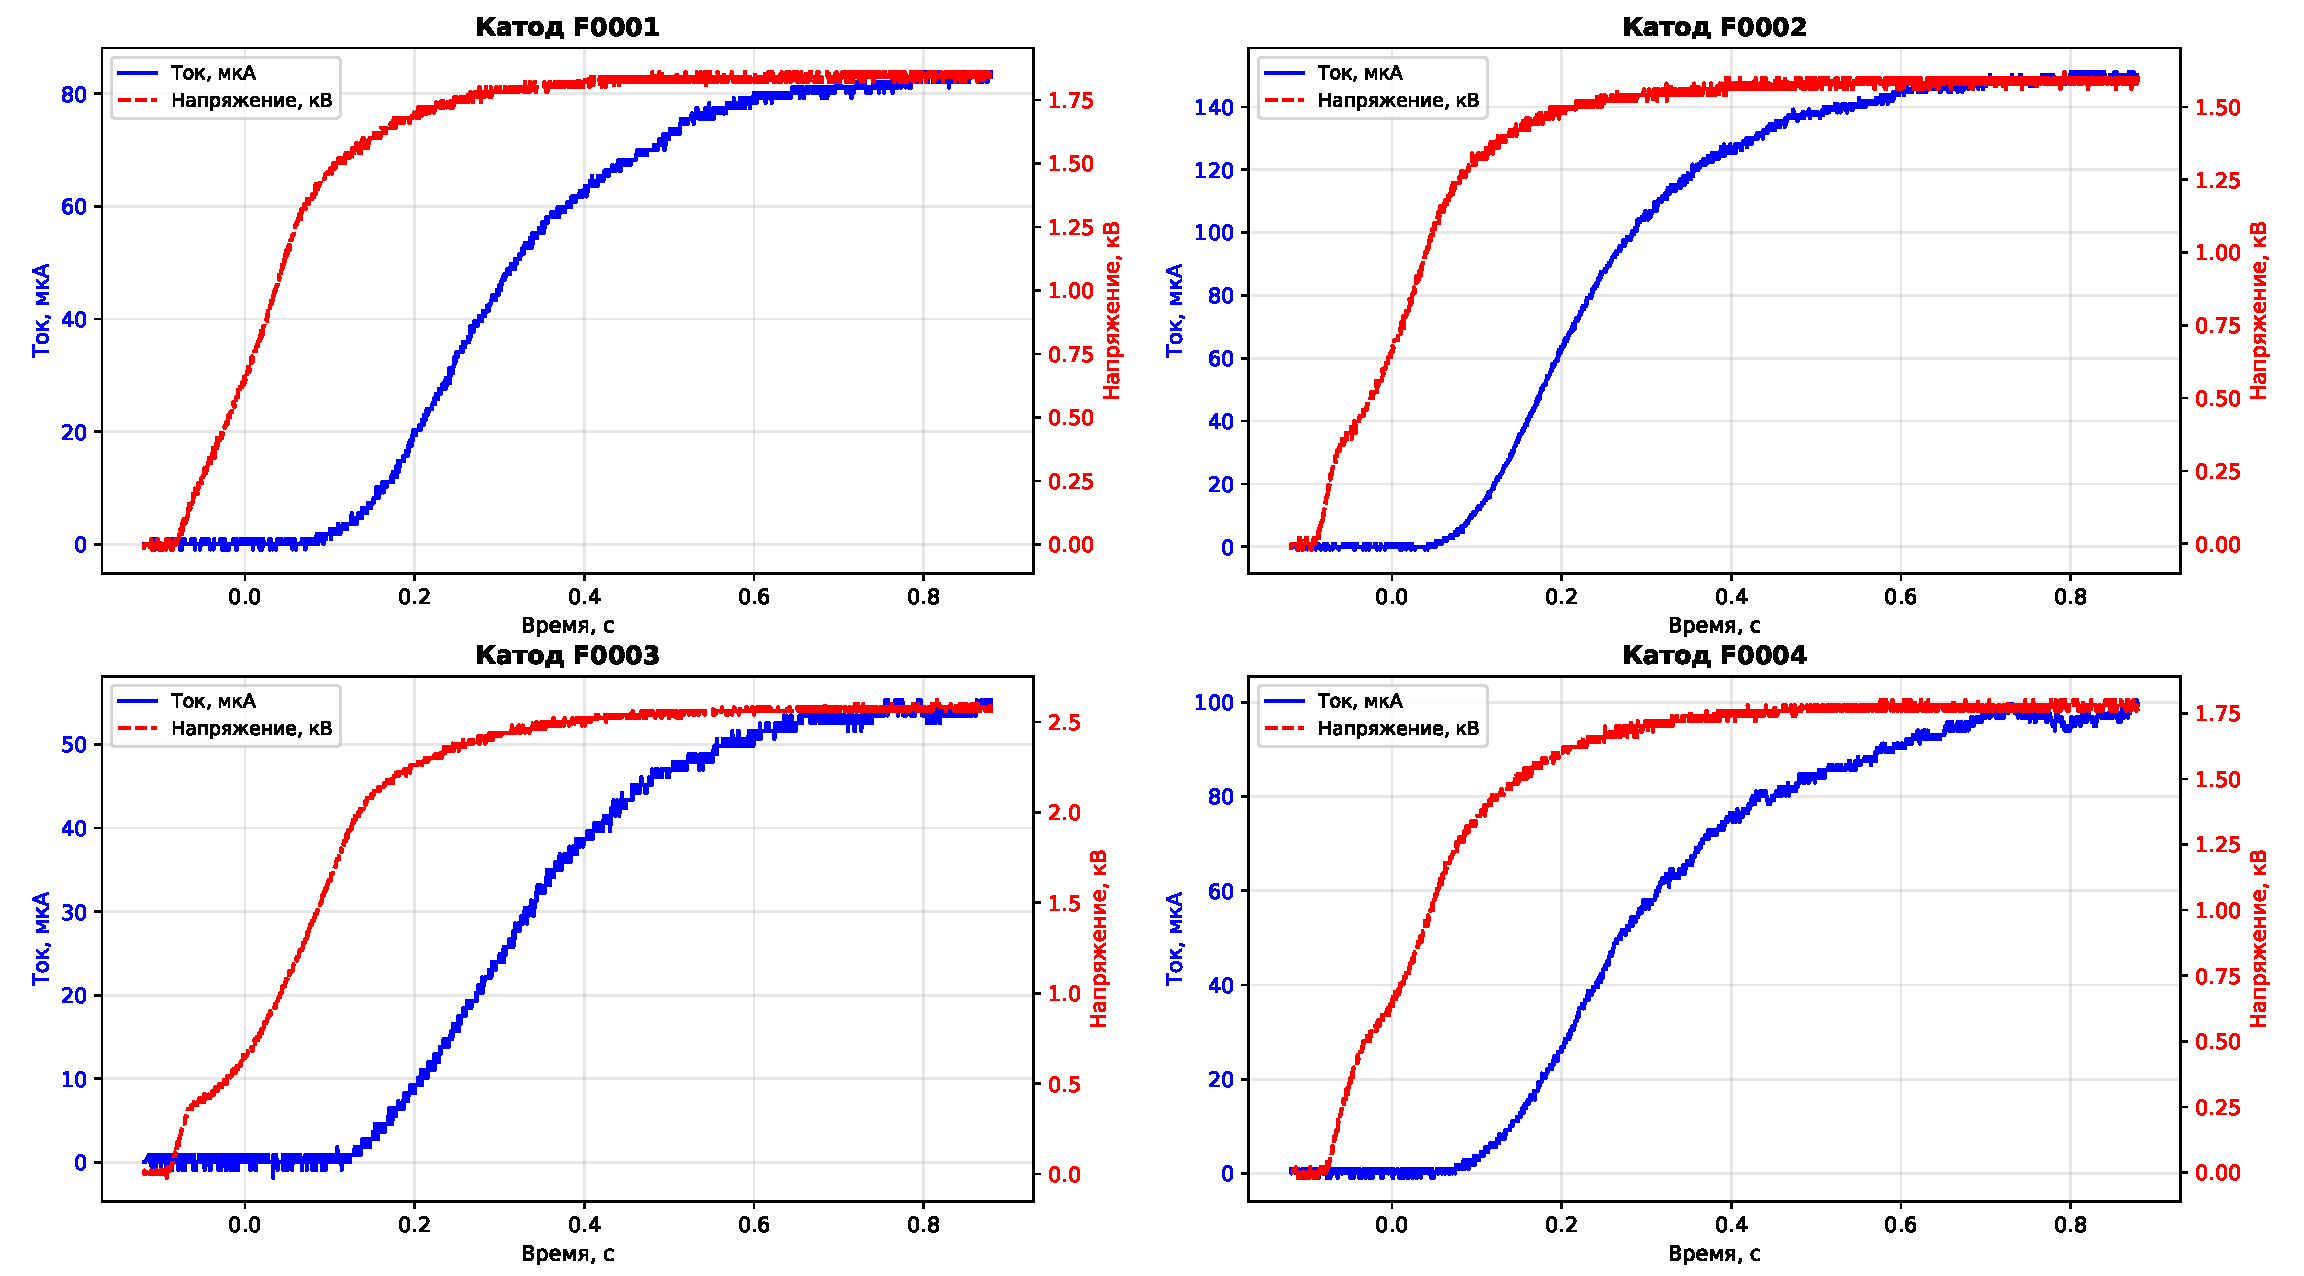
\includegraphics[width=1\textwidth]{4.pdf}
\caption{Переходные процессы тока и напряжения при включении автоэмиссионного катода}
\label{fig:transient}
\end{figure}

Из графиков видно, что установление стационарного значения тока происходит в течение $0{,}2$--$0{,}5$~с. %Наблюдаемый плавный рост или начальный всплеск тока характерен для многоэмиттерных углеродных систем и обусловлен выгоранием наиболее острых, но нестабильных микровыступов, а также десорбцией остаточных газов с поверхности под действием джоулева нагрева.

Для количественной оценки были взяты установившиеся значения тока и напряжения. Результаты представлены в таблице~\ref{tab:steady_state}:

\begin{table}[H]
\centering
\caption{Установившиеся параметры автоэмиссии для исследованных катодов}
\label{tab:steady_state}
\begin{tabular}{|c|c|c|}
\hline
Измерение & $U$, кВ & $I$, мкА \\
\hline
F0001 & 1{,}843 & 82{,}02 \\
F0002 & 1{,}589 & 149{,}03 \\
F0003 & 2{,}575 & 53{,}78 \\
F0004 & 1{,}775 & 97{,}07 \\
\hline
\end{tabular}
\end{table}

% Полученные значения токов (от $53$ до $149$~мкА при напряжениях $1{,}5$--$2{,}5$~кВ) подтверждают высокую эмиссионную способность многоэмиттерных углеродных катодов.

\subsection*{5.1 Обработка данных автоматических измерений в координатах Фаулера--Нордгейма}

Поскольку переходный процесс протекает достаточно медленно, система проходит через последовательность квазистационарных состояний. Это позволяет использовать пары значений $(U(t), I(t))$ из переходного процесса для построения вольт-амперных характеристик в координатах Фаулера--Нордгейма.

На рисунке~\ref{fig:fn_auto_grid} представлены зависимости $\ln(I/U^2)$ от $1/U$ для всех четырёх катодов. 

\begin{figure}[H]
\centering
\includegraphics[width=0.9\textwidth]{transient_FN.pdf}
\caption{ВАХ четырёх катодов в координатах Фаулера--Нордгейма, построенные по данным переходных процессов}
\label{fig:fn_auto_grid}
\end{figure}

Во всех случаях экспериментальные точки с высокой точностью ложатся на прямую линию, что подтверждает полевой (туннельный) механизм эмиссии и применимость уравнения Фаулера--Нордгейма к данным образцам.

\subsection*{5.2 Расчёт форм-фактора $\beta$ и размера эмиссионного центра}

По наклону линейных участков в координатах Фаулера--Нордгейма рассчитывался форм-фактор каждого катода по формуле:
\begin{equation}
    \beta = -\frac{6{,}83 \cdot \varphi^{3/2}}{\tg\alpha},
\end{equation}
где $\varphi = 4{,}7$~эВ (для углерода), а $\tg\alpha$ выражен в кВ. Результаты расчёта $\beta$ представлены в таблице~\ref{tab:beta_auto}.

\begin{table}[H]
\centering
\caption{Расчёт форм-фактора $\beta$ для автоматических измерений}
\label{tab:beta_auto}
\begin{tabular}{|l|c|c|}
\hline
№ ВАХ & $\tg \alpha$, кВ & $\beta$, $10^6$ м$^{-1}$ \\
\hline
Авто 1 & $-24{,}58$ & $2{,}83$ \\
Авто 2 & $-16{,}20$ & $4{,}30$ \\
Авто 3 & $-27{,}11$ & $2{,}57$ \\
Авто 4 & $-15{,}67$ & $4{,}44$ \\
\hline
\end{tabular}
\end{table}

Характерный радиус эмиссионных центров $r$ находился численным решением трансцендентного уравнения (\ref{eq:r_transcendental}) при расстоянии катод--анод $R \approx 1$~мм и коэффициенте формы $k = 1/2$. Результаты оценки размера эмиссионного центра представлены в таблице~\ref{tab:r_auto}.

\begin{table}[H]
\centering
\caption{Оценка характерного радиуса эмиссионного центра}
\label{tab:r_auto}
\begin{tabular}{|l|c|}
\hline
№ ВАХ & Характерный радиус $r$, нм \\
\hline
Авто 1 & $74{,}3$ \\
Авто 2 & $46{,}7$ \\
Авто 3 & $82{,}9$ \\
Авто 4 & $45{,}0$ \\
\hline
\end{tabular}
\end{table}

Полученные значения радиусов ($r \approx 45$--$83$~нм) на два--три порядка меньше геометрического радиуса всего углеродного волокна. Это полностью согласуется с физической моделью, согласно которой эмиссия происходит с отдельных микровыступов (фибрилл) на торцевой поверхности пучка, а не со всей его площади. Также наблюдается ожидаемая обратная корреляция: катоды с большим форм-фактором $\beta$ (например, Авто 4 с $\beta = 4{,}44 \cdot 10^6$ м$^{-1}$ и $r = 45{,}0$ нм) имеют меньший характерный радиус $r$, то есть более острые эмиссионные центры.


\section*{6. Выводы}

В ходе выполнения лабораторной работы было экспериментально исследовано явление автоэлектронной эмиссии на примере многоэмиттерных катодов из углеродных волокон.

\begin{enumerate}
    \item Для исследуемых катодов были сняты вольт-амперные характеристики: одна вручную (с варьированием напряжения) и четыре в автоматическом режиме (путём регистрации квазистационарных точек переходного процесса).
    \item Перестроение зависимостей $I(U)$ в координаты Фаулера--Нордгейма $\ln(I/U^2)$ от $1/U$ показало, что экспериментальные точки с высокой точностью аппроксимируются прямой линией. Это подтверждает полевой (туннельный) механизм эмиссии.
    \item По угловым коэффициентам линейных участков определены форм-факторы катодов. Полученные значения лежат в диапазоне:
    \begin{equation*}
        \beta \approx (2{,}57 \div 4{,}44) \cdot 10^{6}~\text{м}^{-1}.
    \end{equation*}
    \item На основе найденных $\beta$ численно оценены характерные радиусы активных эмиссионных центров:
    \begin{equation*}
        r \approx 45 \div 83~\text{нм}.
    \end{equation*}
    Эти значения согласуются с представлением об эмиссии с отдельных микровыступов на торце пучка волокон.
    \item Наблюдается ожидаемая обратная корреляция между форм-фактором и характерным радиусом: катоды с большим $\beta$ имеют меньший $r$, что означает более сильное локальное усиление электрического поля.
\end{enumerate}







\end{document}